%%%%%%%%%%%%%%%%%%%%%%%%%%%%%%%%%%%%%%%%%
% Short Sectioned Assignment
% LaTeX Template
% Version 1.0 (5/5/12)
%
% This template has been downloaded from:
% http://www.LaTeXTemplates.com
%
% Original author:
% Frits Wenneker (http://www.howtotex.com)
%
% License:
% CC BY-NC-SA 3.0 (http://creativecommons.org/licenses/by-nc-sa/3.0/)
%
%%%%%%%%%%%%%%%%%%%%%%%%%%%%%%%%%%%%%%%%%

%----------------------------------------------------------------------------------------
%	PACKAGES AND OTHER DOCUMENT CONFIGURATIONS
%----------------------------------------------------------------------------------------

\documentclass[paper=a4, fontsize=11pt]{scrartcl} % A4 paper and 11pt font size

\usepackage[T1]{fontenc} % Use 8-bit encoding that has 256 glyphs
%\usepackage{fourier} % Use the Adobe Utopia font for the document - comment this line to return to the LaTeX default
\usepackage[english]{babel} % English language/hyphenation
\usepackage{amsmath,amsfonts,amsthm} % Math packages

\usepackage{graphicx}
\usepackage{indentfirst}

\usepackage{sectsty} % Allows customizing section commands
\allsectionsfont{\centering \normalfont\scshape} % Make all sections centered, the default font and small caps

\usepackage{fancyhdr} % Custom headers and footers
\usepackage{enumerate}
\pagestyle{fancyplain} % Makes all pages in the document conform to the custom headers and footers
\fancyhead{} % No page header - if you want one, create it in the same way as the footers below
\fancyfoot[L]{} % Empty left footer
\fancyfoot[C]{} % Empty center footer
\fancyfoot[R]{\thepage} % Page numbering for right footer
\renewcommand{\headrulewidth}{0pt} % Remove header underlines
\renewcommand{\footrulewidth}{0pt} % Remove footer underlines
\setlength{\headheight}{13.6pt} % Customize the height of the header

\numberwithin{equation}{section} % Number equations within sections (i.e. 1.1, 1.2, 2.1, 2.2 instead of 1, 2, 3, 4)
\numberwithin{figure}{section} % Number figures within sections (i.e. 1.1, 1.2, 2.1, 2.2 instead of 1, 2, 3, 4)
\numberwithin{table}{section} % Number tables within sections (i.e. 1.1, 1.2, 2.1, 2.2 instead of 1, 2, 3, 4)

%\setlength\parindent{0pt} % Removes all indentation from paragraphs - comment this line for an assignment with lots of text

%----------------------------------------------------------------------------------------
%	TITLE SECTION
%----------------------------------------------------------------------------------------

\newcommand{\horrule}[1]{\rule{\linewidth}{#1}} % Create horizontal rule command with 1 argument of height

\title{	
\normalfont \normalsize
\textsc{Skolkovo Institute of Science and Technology} \\ [25pt] % Your university, school and/or department name(s)
\horrule{0.5pt} \\[0.4cm] % Thin top horizontal rule
\huge Application period. Collage \\ % The assignment title
\horrule{0.5pt} \\[0.5cm] % Thick bottom horizontal rule
}

\author{Mariya Popova, Aleksey Grinchuk, Mikhail Shvets} % Your name

\date{\normalsize\today} % Today's date or a custom date

\begin{document}

\maketitle % Print the title


\section{Formulas}

Let $X=\{x_i\}_{i=1}^{W \times H}$ be a collage of $K$ images we are looking for, where each variable $x_i \in \{1,\dots,K\}$ is equal to the number of image we took $i_{th}$ pixel from.

\subsection*{$\alpha$-expansion}

$\alpha$-expansion is an iterative process where we firstly initialize $X$ randomly or set all $x_i = 0$ and on each step select $\\alpha$ and perform expansion step as was discussed on the lectures.

Let us introduce new variable $y_i$ such that
$$y_i = \begin{cases}
1 & x_i^{new} = \alpha\\
0 & x_i^{new} = \alpha \text{ and } x_i^{old} \neq \alpha
\end{cases}$$

Let's look at the pair of vetrices (Fig.\ref{init_graph}). Here we put $\infty$ as $\phi_j(0)$ in case $x_j^{old} = \alpha$, because case $y_j = 0$ should not take place.

\begin{figure}[h!]
\begin{center}
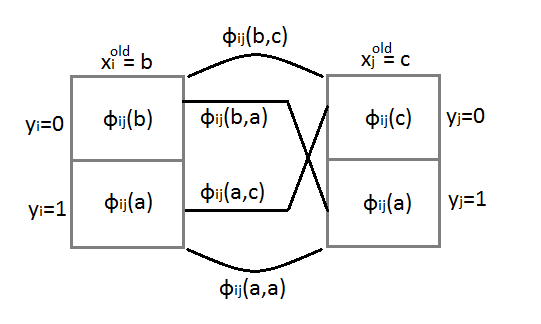
\includegraphics[width=0.45\textwidth]{graph1.png}
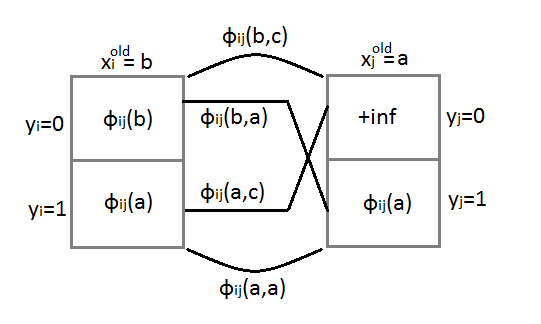
\includegraphics[width=0.45\textwidth]{graph2.png}
\end{center}
\caption{Initial structure}
\label{init_graph}
\end{figure}

To construct a graph we will need to reduce the structure to one where there are only two crossing edges with equal values.
We will use Fig.\ref{graph1} to simplify the notation. Here $*$ means any value and capital letters show values on edges.
\begin{figure}[h!]
\begin{center}
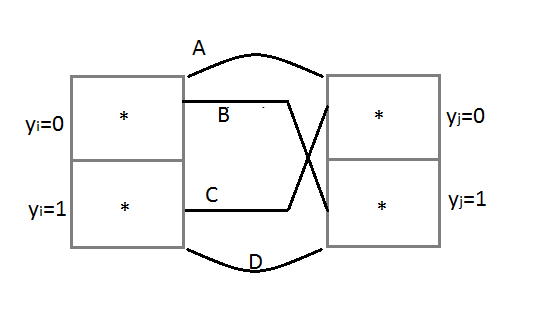
\includegraphics[width=0.7\textwidth]{graph3.png}
\end{center}
\caption{Notation}
\label{graph1}
\end{figure}

Now we perform two steps to achieve our goal (shown in Fig.\ref{graph2})
\begin{figure}[h!]
\begin{center}
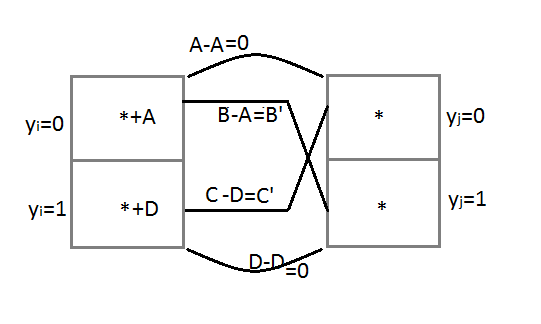
\includegraphics[width=0.45\textwidth]{graph4.png}
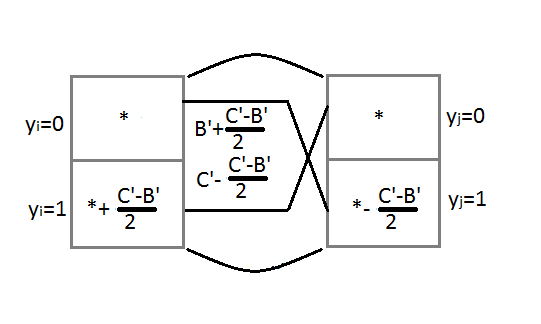
\includegraphics[width=0.45\textwidth]{graph5.png}
\end{center}
\caption{Reduction}
\label{graph2}
\end{figure}

Below we give final formulas to construct the graph. All $\phi_i(y_i)$ and $\phi_{ij}(y_i, y_j)$ are defined in Fig.\ref{init_graph}.

Edge capacity between two variables in lattice:
$$\hat{\phi}_{ij}(0, 1) = \hat{C} = \dfrac{B' + C'}{2} = \dfrac{B-A+C-D}{2} = 
\dfrac{\phi_{ij}(0, 1) - \phi_{ij}(0, 0) + \phi_{ij}(1, 0) - \phi_{ij}(1, 1)}{2}$$

Edge capacities from source to lattice variable and from lattice variable to sink ares initialized with $\phi_i(0)$ and $\phi_i(1)$ and when looking at edge $ij$ are changed according to the rules:
$$\hat{\phi}_{i}(0) = \hat{\phi}_{i}(0) + \phi_{ij}(0, 0)$$
$$\hat{\phi}_{i}(1) = \hat{\phi}_{i}(1) + \phi_{ij}(1, 1) + \dfrac{\phi_{ij}(1, 0) - \phi_{ij}(1, 1) - \phi_{ij}(0, 1) + \phi_{ij}(0, 0)}{2}$$
$$\hat{\phi}_{j}(1) = \hat{\phi}_{j}(1) + \dfrac{\phi_{ij}(0, 1) - \phi_{ij}(0, 0) - \phi_{ij}(1, 0) + \phi_{ij}(1, 1)}{2}$$

\subsection*{$\alpha-\beta$-swap}
$\alpha-\beta$-swap is an alternative iterative process, which chooses $\alpha$ and $\beta$ labels on each step.
Here we introduce a graph of size $| \{ i : x_i = \alpha \text{ or } x_i = \beta \} |$ and binary variables
$$y_i = \begin{cases}
0 & x_i^{new} = \alpha \\
1 & x_i^{old} = \beta
\end{cases}.$$
Again, $y_i$ are introduces only for those $x_i$, where $x_i = \alpha$ or $x_i = \beta$.

We will not need to do any transformation of the graph, because it already satisfies
$$\hat{\phi}_{ij}(0, 0) = \phi_{ij}(\beta, \beta) = 0$$
$$\hat{\phi}_{ij}(0, 1) = \phi_{ij}(\beta, \alpha) = c_{ij}d(\beta, \alpha) = \phi_{ij}(\alpha, \beta) = \hat{\phi}_{ij}(1, 0)$$
$$\hat{\phi}_{ij}(1, 1) = \phi_{ij}(\alpha, \alpha) = 0$$

The only thing, which needs to be handled accurately, is construction of capacities from source to lattice and from lattice to sink:
$$\hat{\phi}_i(0) = \phi_i(\beta) + \sum\limits_{k: x_k \neq \alpha \text{ and } x_k \neq \beta} \phi_{ik}(\beta, x_k)$$
$$\hat{\phi}_i(1) = \phi_i(\alpha) + \sum\limits_{k: x_k \neq \alpha \text{ and } x_k \neq \beta} \phi_{ik}(\alpha, x_k)$$

\end{document}
